Adesso vediamo le proprietà dei quark e dei gluoni da un altro punto di vista. 
\subsection{Esperimento di scattering}
\begin{itemize}
    \item Vogliamo sapere se il bersaglio è un semplice oggetto puntiforme, e se non lo è dobbiamo capire come sondare la sua struttura. 
    \item Per fare ciò ci serviamo di esperimenti di scattering. Potremmo fare scattering di Rutherford (1911) ma utilizzò particelle $\alpha$ e non riusci neanche a vedere la dimensione del nucleo (di oro). Infatti successivamente tra 1950-1960 Hofstadter arrivò alla struttura nucleare con elettroni in nuclei di $H/D/He$ e infine tra 1965-1980 (SLAC/CERN) con elettroni siamo arrivati alla materia adronica cioè i quark.
    \item Preferiamo usare come sonda una particella elementare, normalmente un elettrone, perché, oltre ad essere semplici da produrre, vogliamo scegliere noi la energia della sonda e soprattutto perché così siamo "sicuri" che il proiettile sia elementare e tutti gli effetti di non-elementarietà sono dovuti esclusivamente al bersaglio.
    \item Dunque in ordine:
    \begin{enumerate}
        \item Si sceglie una sonda (e.g. elettrone)
        \item Si studia lo scattering $e^-$-target 
        \item Si misura la sezione d'urto di $e^-T$, la distribuzione angolare di $e^-$ e si rivelano stati eccitati o lo stato finale del sistema adronico (scattering anelastico)
    \end{enumerate}
    \item Il modo di procedere è:
    \begin{enumerate}
        \item Si studia la cinematica. Con cinematica intendiamo le equazioni che seguono dalla conservazione di momento angolare e massa. Dopo aver imposto i vincoli cinematici si studia la \textit{dinamica}. 
        \item Calcoliamo la $\sigma(e^-T)$ per nuclei puntuali in elettrodinamica classica (formula di Rutherford).
        \item Si fa lo stesso per la meccanica quantistica con elettroni ($s=\frac12$) e nuclei puntuali (formula di Mott)
        \item Si rivelano \textit{deviazioni} da questi modelli. Così derivo informazioni sulla struttura nucleare
        \item Formulo una nuova teoria, poi vado a distanze ancora più piccole ($Q^2$ maggiore) e vedo se la nuova teoria regge o ci sono altre deviazioni e ripeto, potenzialmente fino all'infinito.
    \end{enumerate}
\end{itemize}
\begin{figure}[H]
    \centering
    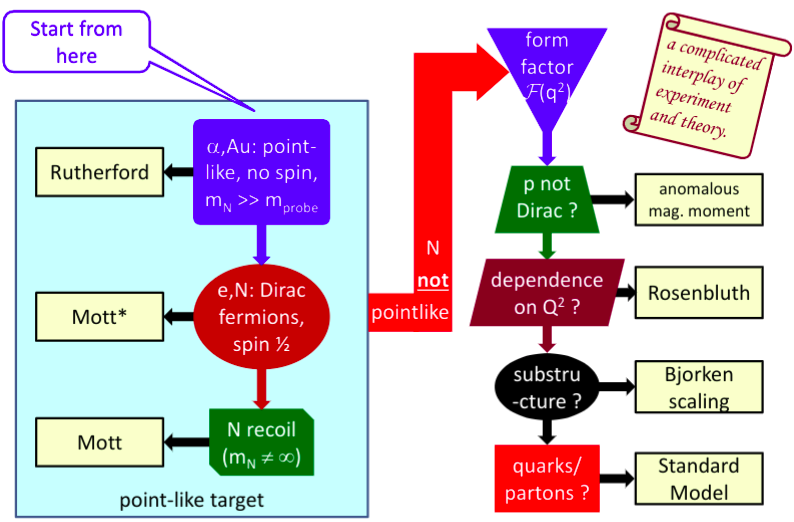
\includegraphics[width=0.7\textwidth]{immagini/fig_treasure_map_scattering}
    \caption{Mappa del tesoro dello scattering.}
    %\label{}
\end{figure}
\subsection{Modello a gas di Fermi}
\begin{itemize}
    \item I nuclei sono stati legati di protoni e neutroni. Il gas di Fermi è un semplice modello.
    \item I protoni e i neutroni sono identici a meno della carica: sono delle sfere con una certa massa; sono fermioni; sono legati all'interno del nucleo, altrimenti sono liberi di muoversi. 
    \item Non consideriamo interazione elettromagnetica, solo nucleare dunque $N=Z=\frac A2$ ed impulso ed energia di Fermi sono uguali per protoni e neutroni (in approssimazione migliore sono differenti gli impulsi). 
    \item Per il principio di indeterminazione ogni $p$ ed $n$ occupano un volume $V=(2\pi\hbar)3$ nello spazio delle fasi.
    \item Dunque abbiamo una buca ben definita identica per protoni e neutroni, e viene rispettata la statistica di Fermi dunque due $p/n$ per livello di energia (con spin opposto).
    \item Da queste approssimazioni possiamo fare dei calcoli semplici:
    \begin{gather*}
    n_n^\uparrow=n_n^\downarrow=n_p^\uparrow=n_p^\downarrow=\frac N2=\frac Z2=\frac A4=\\
    =\frac{[V\_{space}V\_{imp}]\_{TOT}}{[V\_{space}V\_{imp}]\_{ciascuna particella}}=\frac{\frac43\pi r_0^3A\times\frac43\pi p_F^3}{(2\pi\hbar)^3}=\frac{2Ar_0^3p_F^3}{9\pi^2\hbar^3}\implies\\
    \implies N=Z=\frac A2=\frac{4Ar_0^3p_F^3}{9\pi^2\hbar^3}\implies p_F=\frac\hbar{r_0}\sqrt[3]{\frac{9\pi}8}\underset{r_0\approx1.2\,\text{fm}}{\implies}
    \begin{cases}
    p_F\approx250\,\MeV\\
    E_F^{\text{kin}}=\frac{p_F^2}{2m}\approx33\,\MeV
    \end{cases}
    \end{gather*}
    dove il valore di $r_0$ viene da fit del fattore di forma (vedi dopo) e per $E^{\text{kin}}_F$ si è considerata approssimazione non relativistica. 
    \item In conclusione: $V\_{space}\approx\frac43\pi r_0^3A\implies r\_{nucl}\propto A^{1/3}$, impulso ed energia di Fermi non dipendono da $A$ e ad un largo $p_F$ corrisponde bassa energia cinetica ed infine quando $p/n$ sono colpiti da una sonda ($e^\pm/\nu$), se l'energia della sonda è superiore a 30 MeV, si ignora il moto di Fermi.  
\end{itemize}
\subsection{Scattering di Rutherford}
\begin{itemize}
    \item L'esperimento fu eseguito a Manchester nel 1908-1913. Consiste in particelle $\alpha$ contro un bersaglio di oro $Au$.
    \item Propose un modello diverso da quello di J.J. Thompson.
    \item Fu il primo esperimento di scattering di particelle, infatti è la nascita della fisica nucleare.
    \item Dunque si mandarono queste particelle $\alpha$ su un foglio di oro con energia cinetica di qualche MeV. Qualche volta l'angolo di scattering era maggiore di 90$^\circ$ che nella pratica è un evento molto raro ma impossibile se la materia fosse effettivamente omogenea come nel modello di Thompson. L'unica possibile spiegazione è che la materia in realtà è concentrata in piccoli corpi pesanti, i nuclei. Dunque la materia è essenzialmente vuota.
    \item Come modelliamo lo scattering? Rutherford provo con una diffusione a due corpi. Chiaramente solo contributo elettrostatico non relativostico e senza meccanica quantistica. Fu un successo.
    \item Un punto chiave è che il nucleo è abbastanza piccolo da essere visto puntiforme (e con tutta la sua carica) dalla particella $\alpha$ (teorema di Gauss, primo capitolo).
    \item Tuttavia la materia è neutra, ma il fatto è che gli elettroni sono molto leggeri e non possono fermare o deflettere le particelle $\alpha$ perché $m_\alpha\approx8000m_e$.
\end{itemize}
    \subsubsection{Calcolo della sezione d'urto}
    \begin{figure}[H]
        \centering
        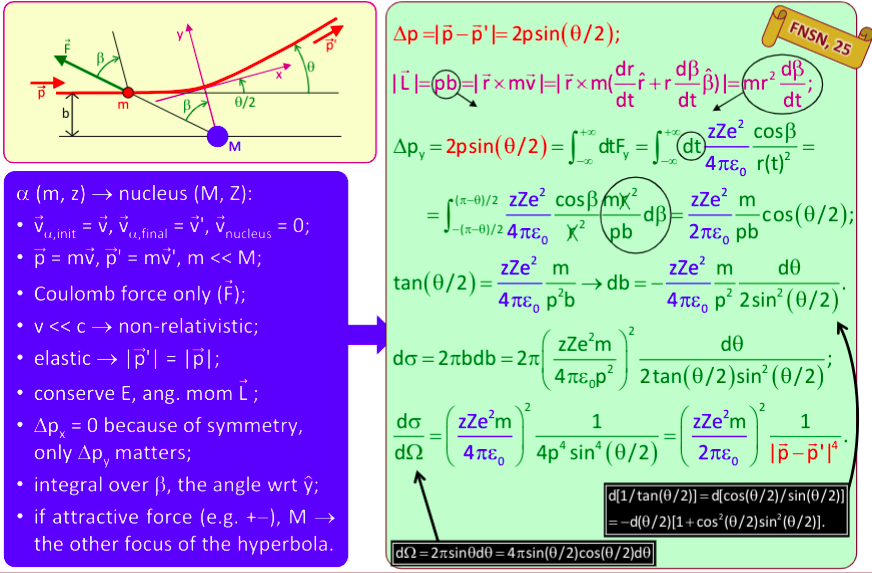
\includegraphics[width=\textwidth]{immagini/fig_rutherford_math.png}
        \caption{$\beta$ è l'angolo tra la particella e l'asse di simmetria (che passa per il punto di minimo approccio).}
        %\label{}
    \end{figure}
    \begin{itemize}
    \item Se la forza è attrattiva la sezione d'urto è uguale perché cambia solo
        \begin{equation*}
    \vec F\to -\vec F\implies\vartheta\to-\vartheta
    \end{equation*}
    \item Adesso troviamo espressione esplicita per la $r\_{min}$. Cominciamo una particella con $b=0\implies \vartheta=\pi$. Avremo $d_0=r\_{min}(b=0)$ dato da
    \begin{equation*}
    \frac12mv^2=\frac{zZe^2}{4\pi\varepsilon_0d_0}\implies d_0=\frac{zZe^2}{2\pi\varepsilon_0mv^2}\implies \tan\qty(\frac\vartheta2)=\frac{d_0}{2b}
    \end{equation*}
    Per trovare $d$ ($b\neq0$) usiamo conservazione di $\vec L$ ed $E$ (dove $v_0$ è la velocità in $d$)
    \begin{equation*}
        \begin{cases}
        mbv=mdv_0\to \frac{v_0}v=\frac bd\\
        \frac12mv^2=\frac12mv_0^2+\frac{zZe^2}{4\pi\varepsilon_0d}=\frac12mv_0^2+\frac12mv^2\frac{d_0}d
        \end{cases}\implies\qty(\frac bd)^2=\qty(\frac{v_0}v)^2=1-\frac{d_0}d\implies 
    \end{equation*}
    \begin{equation*}
        \implies d^2-dd_0-b^2=0\implies d=\dots=\frac{d_0}2\qty(1+\frac1{\sin(\frac\vartheta2)})\implies \dv{\sigma}{\Omega}= \frac{d_0^2}{16\sin^4\qty(\frac\vartheta2)}\overset{\vartheta\to0}{\longrightarrow}\frac{d_0^4}{\vartheta^4}
    \end{equation*}
    \begin{figure}[H]
        \centering
        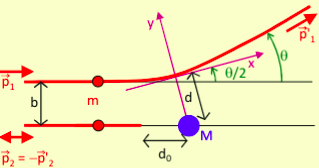
\includegraphics[width=0.6\textwidth]{immagini/fig_ruth_b_nullo.png}
        %\caption{}
        %\label{}
    \end{figure}
    \item Questi calcoli non sono difficili da fare matematicamente, la vera difficoltà è affermare se la materia è omogenea o granulare e vuota.
    \item A grandi $b$ corrispondono piccoli $\vartheta$ a cui corrisponde una divergenza della sezione d'urto, poi comunque non diverge perché c'è un limite dato dalla presenza di altri nuclei di oro. 
    \item Nel 1909 trovarono eventi di backscattering che misero in crisi il modello di Thomson. Era comunque inconsistente perché elettroni che accelerano emettono radiazione elettromagnetica e dovrebbero collassare nel nucleo. Dopo la nascita della MQ comunque la sezione d'urto rimase la stessa\footnote{la prof dice "per caso", Greco dice perché la $\alpha$ ha spin nullo}.
\end{itemize}
\subsubsection{Raggio nucleare}    
Quanto è grande il nucleo? Se la particella $\alpha$ ha una traiettoria esterna, essa non può sondare la sua \textit{ipotetica} struttura interna. Rutherford arrivò a $r\approx10^{-14}$ m. Per andare oltre servono sonde con $E\_{kin}\approx30$ MeV.
\begin{itemize}
    \item $b$ ed $r\_{min}$ non possono essere misurati direttamente per ciascun evento, ma la legge puntiforme di Rutherford (rpl) lega $b\leftrightarrow\vartheta$ infatti a piccoli parametri d'urto corrispondono grandi angoli.
    \item Il teorema di Gauss predice una deviazione da rpl quando l'energia cinetica delle $\alpha$ è grande. Avendo un $r\_{min}<R\_N$ si avrà schermaggio dunque degli angoli $\vartheta$ più piccoli.
    \item nel 1961 fecero una misura di scattering $\alpha$ contro piombo mettendosi a $\vartheta=60^\circ$ ed osservarono una deviazione da rpl per energie superiori a 25 MeV (dunque nucleo non è puntiforme).
    \item Ad angoli grandi, se il bersaglio è puntiforme la sezione d'urto è grande, se invece è esteso la sezione d'urto è minore. Non è proprio chiaro scritto così ma è legato ai precedenti punti. 
\end{itemize}
\subsection{Cinematica}
Come già detto la nostra sonda è una particella elementare e il nostro bersaglio è in generale un complesso sistema adronico. Nello stato finale si avrà la sonda invariata mentre il nucleo in generale cambia:
\begin{enumerate}
    \item Scattering elastico: il nucleo rimane nello stato fondamentale.
    \item Eccitazione: il nucleo nello stato finale si trova in uno stato eccitato.
    \item Nuovo sistema adronico, con $n$ particelle.
\end{enumerate}
L'idea è capire/studiare la struttura degli adroni osservando lo scattering.
\subsubsection{Scattering elastico}
\begin{itemize}
    \item Consideriamo $e^-N\to e^-N$, con nucleo inizialmente a riposo. Allora avremo che l'energia finale dell'elettrone è (da consevazione di quadrimpulso)
    \begin{equation*}
        E'=\frac E{1+\frac EM\qty(1-\cos\vartheta)}=\frac E{1+\frac{2E}{M}\sin^2\frac\vartheta2}\approx \abs{\vec p'}
    \end{equation*}
    \begin{figure}[H]
        \centering
        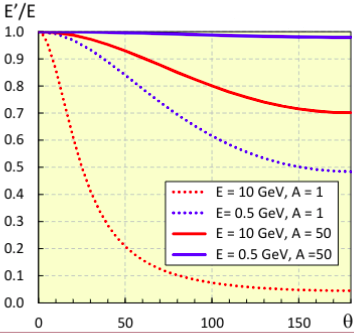
\includegraphics[width=0.6\textwidth]{immagini/fig_frac_energy_scatt.png}
        \caption{Grafico della frazione di energia portata via dall'elettrone. Quando l'energia iniziale è alta e il nucleo è piccolo (A=1) viene trasferita molta energia al nucleo a grandi angoli. Se $\frac EM$ è piccolo, allora $E'\approx E\implies p\_H\approx0$ cioè non rincula ed è indipendente da $\vartheta$.}
        %\label{}
    \end{figure}
    \item Dunque nota l'energia iniziale e fissata la massa $M$ del nucleo, lo stato finale è definito da \textit{una variabile indipendente} $E'$ o $\vartheta$.
    \item Per il calcolo esplicito bisogna considerare la conservazione del quadrimpulso prima e dopo lo scattering, e poi fare il quadrato e sottrarre le due equazioni isolando l'energia del nucleo post-scattering (una per conservazione di energia e l'altra per l'impulso).
    \item Consideriamo l'impulso trasferito $\vec q = \vec p - \vec p'$. Se $E/M$ è piccolo, allora $p'=p\implies \abs{\vec q}=2\abs{\vec p}\sin\frac\vartheta2$. 
    \item C'è anche la controparte relativistica, ossia il quadrivettore $q=(E-E',\vec p-\vec p')$. 
    \begin{equation*}
    -q^2=-(2m_e^2-2EE'+2\abs{\vec p}\abs{\vec p'}\cos\vartheta)\approx4EE'\sin^2\frac\vartheta2=Q^2>0
    \end{equation*}
    Possiamo ricavare una relazione per $Q^2$ nel seguente modo:
    \begin{equation*}
        E'=\frac{EM}{M+2E\sin^2\frac\vartheta2}=\frac{EM}{M+\frac{Q^2}{2E'}}=\frac{2EE'M}{2E'M+Q^2}\implies 2EM=E'M+Q^2\implies
    \end{equation*}
    \begin{equation*}
        \implies Q^2=2M(E-E')\qquad E'=E-\frac{Q^2}{2M}
    \end{equation*}
    \item Vediamo i casi cinematici limite:
    \begin{enumerate}
        \item $\vartheta=0$: $E'=E$, $Q^2=0$.
        \item $\vartheta=\pi$: $E-E'=E\frac{M+2E}{M+2E}-\frac{EM}{M+2E}=\frac{2E^2}{M+2E}$, quindi se $E\ll M$ allora $E-E'\approx E\implies E'\approx0$ 
    \end{enumerate}
    \begin{figure}[H]
        \centering
        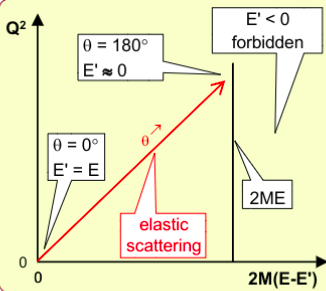
\includegraphics[width=0.6\textwidth]{immagini/fig_q_2_elastic.png}
        \caption{Grafico di $Q^2$ in funzione di $2M(E-E')$: solo un segmento è permesso.}
        %\label{}
    \end{figure}
\end{itemize}
\subsubsection{Perché usare $\abs{\vec q}$ o $Q^2$?}
La variabile $\vec q$ (o $Q^2$ in regime relativistico) è molto importante
\begin{itemize}
    \item È legata alla lunghezza d'onda di De Broglie della sonda $\slashed\lambda=\frac\hbar{\abs{\vec q}}$. Rappresenta la scala dello scattering, ossia strutture più piccole di $\slashed\lambda\sim\frac1{\abs{\vec q}}$ non possono essere viste dalla sonda.
    \item Questo viene dal principio di indeterminazione $\Delta p\Delta x\geq \frac\hbar2$.
    \item A grandi $\abs{\vec q}$ corrispondono grandi energie, ma l'opposto in generale non è vero: esistono processi ad alta energia e grandi distanze.
    \item La ricerca di scale inferiori porta inevitabilmente a maggiori $Q^2$ e dunque a grandi energie (soldi e risorse). 
\end{itemize}
\subsubsection{Scattering inelastico}
Consideriamo il caso $lN\to l'H$. Sia $p$ il quadrimpulso dell'elettrone, $P$ il quadrimpulso del nucleo, $p'$ il quadrimpulso dell'elettrone dopo lo scattering e $p_H$ il quadrimpulso del nucleo dopo lo scattering. Definiamo/riscriviamo delle variabili Lorentz-invarianti:
\begin{itemize}
    \item $\nu=q\frac PM=E-E'$ è l'energia persa dall'elettrone.
    \item $Q^2=-q^2=2(EE'-pp'\cos\vartheta)-2m^2\approx4EE'\sin^2(\frac\vartheta2)$ 
    \item $x=\frac{Q^2}{2M\nu}$ è la "x di Bjorken" e corrisponde alla frazione di quadrimpulso dell'adrone portata dal partone interagente.
    \item $y=\frac{q\cdot P}{p\cdot P}=\frac\nu E$ è la frazione di energia persa dal leptone nel riferimento del bersaglio.
    \item $W^2=(p\_H)^2=(p+q)^2=M^2-Q^2+2M\nu$ è il quadrato della massa del sistema adronico finale. Se $W=M$ allora si ha scattering elastico.
    \item $s=(q+P)^2=(p'+p\_H)^2\approx M(M+2E)$ è il quadrato dell'energia nel centro di massa.
\end{itemize}
\begin{figure}[H]
    \centering
    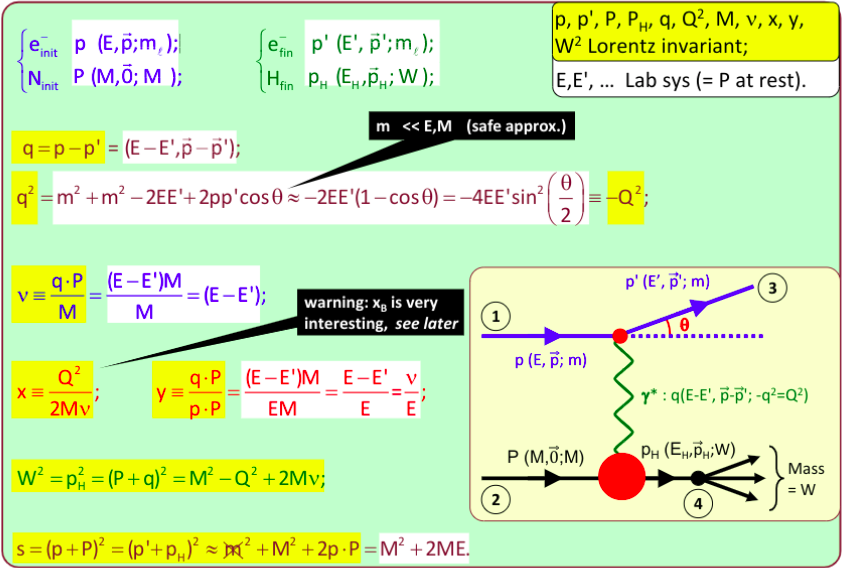
\includegraphics[width=\textwidth]{immagini/fig_conti_kinem.png}
    %\caption{}
    %\label{}
\end{figure}
\begin{itemize}
    \item Nel caso elastico $eN\to eN$, $\nu$ e $Q^2$ NON sono indipendenti:
    \begin{equation*}
    W^2=M^2=(P+q)^2=M^2-Q^2+2M\nu\implies Q^2=2M\nu\implies\frac{Q^2}{2M\nu}=x=1
    \end{equation*}
    \item Dunque ovviamente nel caso elastico c'è solo una variabile indipendente ($E'$ o $\vartheta$), mentre nel caso inelastico ce ne sono due:
    \begin{equation*}
        Q^2=M^2+2M\nu-W^2=2M\nu-(W^2-M^2)\leq2M\nu\implies x\leq1
    \end{equation*}
    se $W$ non è fissato, $Q^2$ e $\nu$ sono indipendenti.
    \item Si scelgono per convenienza le due variabili indipendenti da analizzare, e.g. $(E',\vartheta)$, $(Q^2,\nu)$, $(x,y)$.
\end{itemize}
\subsubsection{Deep inelastic scattering (DIS)}
Torniamo al piano $Q^2,\nu$.
\begin{itemize}
    \item Entrambi sono Lorentz-invarianti.
    \item $Q^2=4EE'\sin^2\frac\vartheta2\geq0$ dunque stiamo nel primo quadrante.
    \item $\nu=E-E'\implies0\leq\nu\leq E$ dunque solo una banda è permessa.
    \item $x=\frac{Q^2}{2M\nu}\leq1\implies 0\leq x\leq1$ dunque solo il "triangolo basso" è permesso.
    \item $y=\frac\nu E\implies0\leq y\leq1$.
    \item $W^2=M^2-Q^2+2M\nu$ la bisettrice $x=1$ definisce lo scattering elastico dove $W=M$. Lungo la bisettrice solo $\vartheta$ varia: $\vartheta=0\implies Q^2=\nu=0$.
    \item Il luogo dei punti $W'^2=$cost sono linee parallele alla bisettrice, alcune di loro definiscono gli stati eccitati.
    \item A distanze maggiori dalla bisettrice abbiamo DIS e potenzialmente nuova fisica.
    \begin{figure}[H]
        \centering
        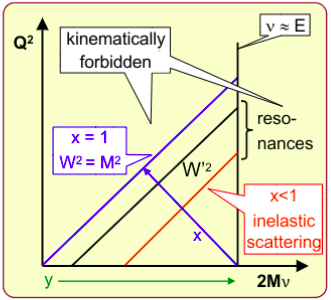
\includegraphics[width=0.6\textwidth]{immagini/fig_dis.png}
        %\caption{}
        %\label{}
    \end{figure}
\end{itemize}
\subsubsection{Riassunto cinematica}
\begin{figure}[H]
    \centering
    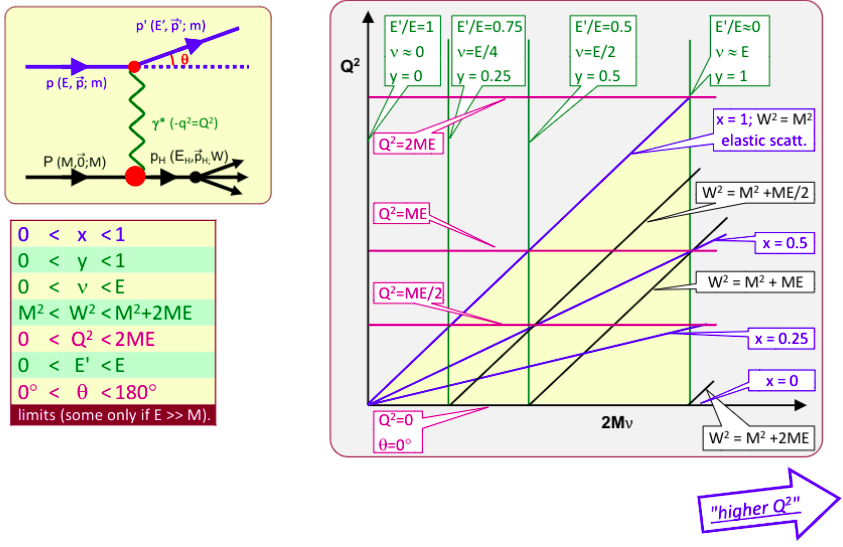
\includegraphics[width=\textwidth]{immagini/fig_kin_summary_hadron.png}
    %\caption{}
    %\label{}
\end{figure}
\subsection{Scattering elastico $eN$: Rutherford + MQ}
Negli anni 20 entrò in gioco la meccanica quantistica. 
\begin{itemize}
    \item La formula di Rutherford funziona anche in questo caso, considerando il caso non relativistico e la approssimazione di Born.
    \item Il potenziale è comunque coloumbiano.
    \item Gli stati iniziali e finali delle particelle sono onde piane.
    \item Trascuriamo il rinculo.
    \item Il potenziale all'infinito non contribuisce a causa degli altri nuclei.
    \item Vediamo il calcolo:
    \begin{gather*}
        V(r)=-\frac{zZ\alpha}r;\;\vec q=\Delta p=\vec p-\vec p';\;q=\abs{\vec q}=2p\sin\frac\vartheta2\\
        \psi_i=\frac1\Phi e^{i\vec p\cdot \vec r};\;\psi_f=\frac1\Phi e^{i\vec p'\cdot \vec r};\; \dv{n}{E'}=\frac{4\pi p'^2\Phi}{(2\pi)^3v'}\\
        M\_{fi}=\braket{\psi_f}{V}{\psi_i}=\frac1\Phi\int e^{-i\vec p'\cdot\vec r}V(r)e^{i\vec p\cdot\vec r}\dd^3r=\\
        =-\frac1\Phi\iiint \frac{zZ\alpha}re^{i\vec q\cdot\vec r}r^2\dd r\dd\Omega=-\frac{4\pi}\Phi\frac{zZ\alpha}{q^2}\\
        \implies \dv{\sigma}{\Omega}=\frac1{4\pi}\qty[2\pi\abs{M\_{fi}}^2\dv{n}{E'}\frac\Phi{v'}]\underset{\begin{subarray}{c}
            v'\to c=1\\
            p'=E'
         \end{subarray}}{\longrightarrow}\frac12\abs{\frac{4\pi}\Phi\frac{zZ\alpha}{q^2}}^2\frac{\Phi E'^2}{2\pi^2}\Phi=\frac{4z^2Z^2\alpha^2E'^2}{q^4}
    \end{gather*}
    stesso risultato!
    \item Tuttavia lo scattering $\alpha-$Nucleo ha luogo due particelle non elementari, dunque sostituiamo $\alpha$ con elettrone. 
    \item La dinamica dello scattering $eN$ può essere descritta dalla formula di Rutherford con un aggiustamento dovuto a Mott\footnote{L'asterisco indica che stiamo approssimando trascurando il rinculo del nucleo.}:
    \begin{equation*}
    \dv{\sigma}{\Omega}\_{Mott*}=\dv{\sigma}{\Omega}\_{Ruth}\times\qty(1-\beta^2\sin^2\frac\vartheta2)\underset{\beta=\frac{\abs {\vec p}}{E}\to1}{\longrightarrow}\dv{\sigma}{\Omega}\_{Ruth}\cos^2\frac\vartheta2=\frac{4Z^2\alpha^2E'^2}{q^4}\cos^2\frac\vartheta2
    \end{equation*}
    \item Come la formula di Rutherford, la sezione d'urto di Mott trascura le dimensioni del nucleo, se ci sono (e anche il rinculo quando mettiamo *).
    \item Al contrario della formula di Rutherford, qui si tiene conto dello spin ($\frac12$) degli elettroni.
\end{itemize}
\subsubsection{Elicità}
\begin{itemize}
    \item Il fattore $\cos^2\frac\vartheta2$ nella sezione d'urto di Mott viene dalla equazione di Dirac. Lo si capisce considerando il caso estremo $\vartheta\sim\pi$.
    \item Per particelle relativistiche ($\beta\to1$) l'elicità $h$ (proiezione di spin su impulso) è conservata:
    \begin{equation*}
    h=\frac{\vec s\cdot \vec p}{\abs{\vec s}\abs{\vec p}}
    \end{equation*}
    \item La conservazione richiede uno spin flip dell'elettrone tra stato iniziale e finale, perché anche l'impulso flippa a 180$^\circ$.
    \item Però in questa condizione, il momento angolare NON si conserva se il nucleo non assorbe la variazione di spin (e.g. perché è a spin nullo). Dunque lo scattering a $\vartheta\approx\pi$ è proibito.
    \item Il fattore $\cos^2\frac\vartheta2$ nella formula di Mott è connesso allo spin e descrive la parte magnetica della interazione. Quindi questo termine serve ad annullare la sezione d'urto altrimenti non si conserverebbe il momento angolare.
    \item Se invece il target ha spin, la proiezione dello spin dell'elettrone può cambiare perché la conservazione del momento angolare può essere compensata dal cambio nella direzione dello spin del bersaglio. In questo caso lo scattering a 180$^\circ$ è possibile.
    \begin{figure}[H]
        \centering
        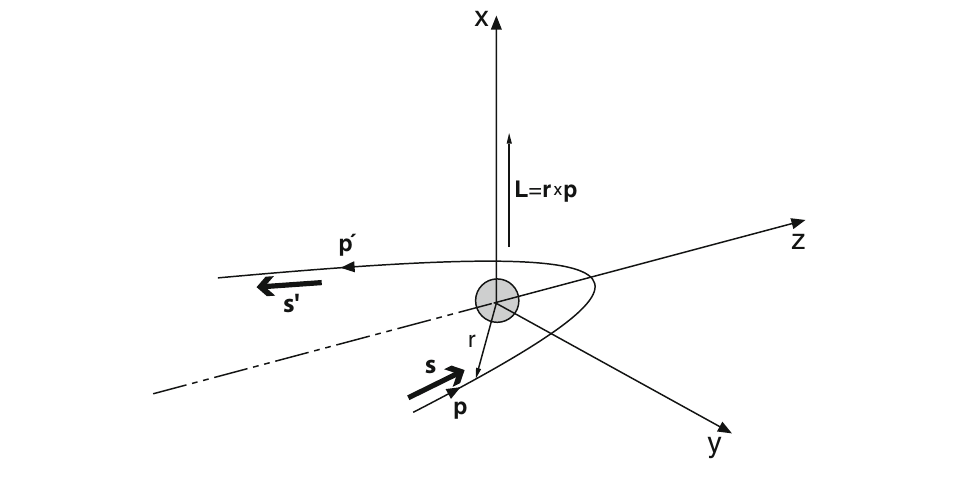
\includegraphics[width=0.8\textwidth]{immagini/fig_elic_mott.png}
        \caption{L'elicità si conserva nel limite $\beta\to1$. Questo significa che la proiezione dello spin lungo $z$ deve cambiare di segno nello scattering a 180$^\circ$. Questo è impossibile se il bersaglio è a spin nullo per conservazione del momento angolare.}
        %\label{}
    \end{figure}
\end{itemize}
\subsubsection{L'esperimento}
L'esperimento è consistente con la cinematica dello scattering elastico? Abbiamo i dati $e+\,^{12}C$.
\begin{figure}[H]
    \centering
    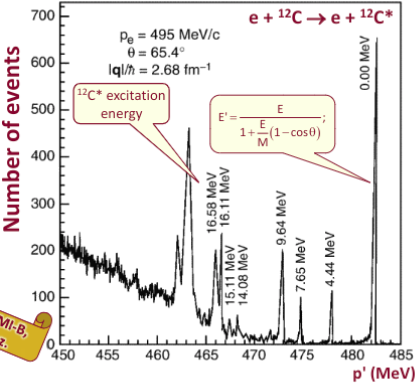
\includegraphics[width=0.6\textwidth]{immagini/fig_plot_eN_scatt.png}
    %\caption{}
    %\label{}
\end{figure}
Il plot dei numeri di eventi con $E\_{in}$ e $\vartheta$ fissato, mostra vari picchi:
\begin{enumerate}
    \item Il più grande è il picco elastico come ci aspettiamo ($E'\approx p'=482$ MeV)
    \item Si ha una struttura "ricca" a causa dello scattering anelastico in cui si porta il carbonio a stati eccitati.
\end{enumerate}
 